\chapter{Defining the problem}

\section{Iris flowers}
We are given sepal length, sepal width, petal length, petal width and our goal is to classify whether an iris flower is any of the following:

\begin{enumerate}
    \item Iris Setosa, see figure \ref{fig:setosa}. The image was taken from the Wikipedia article for Iris setosa~\cite{setosa}.
    \item Iris Versicolour, see figure \ref{fig:versicolour}. The image was taken from the Wikipedia article for Iris versicolour ~\cite{versicolor}.
    \item Iris Virginica, see figure \ref{fig:virginica}. The image was taken from the Wikipedia article for Iris Virginica ~\cite{virginica}.
\end{enumerate}
\begin{figure}
    \centering
    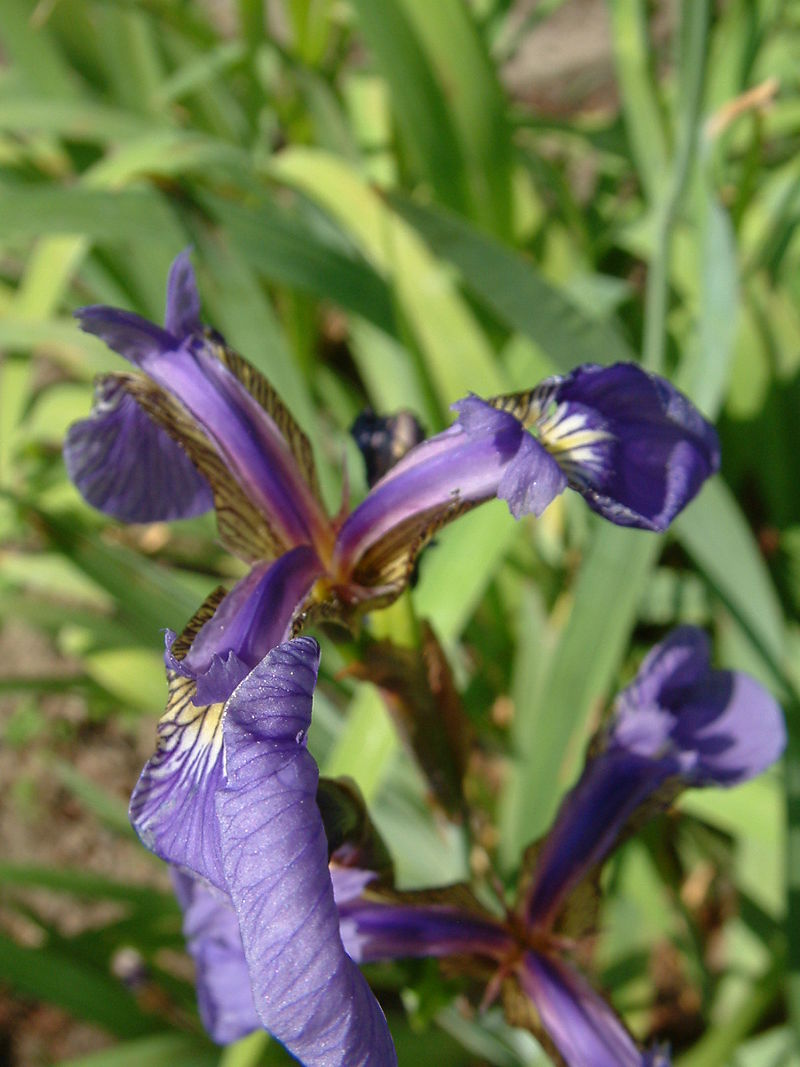
\includegraphics[scale=0.2]{setosa}
    \caption{Iris Setosa}
    \label{fig:setosa}
\end{figure}
\begin{figure}
    \centering
    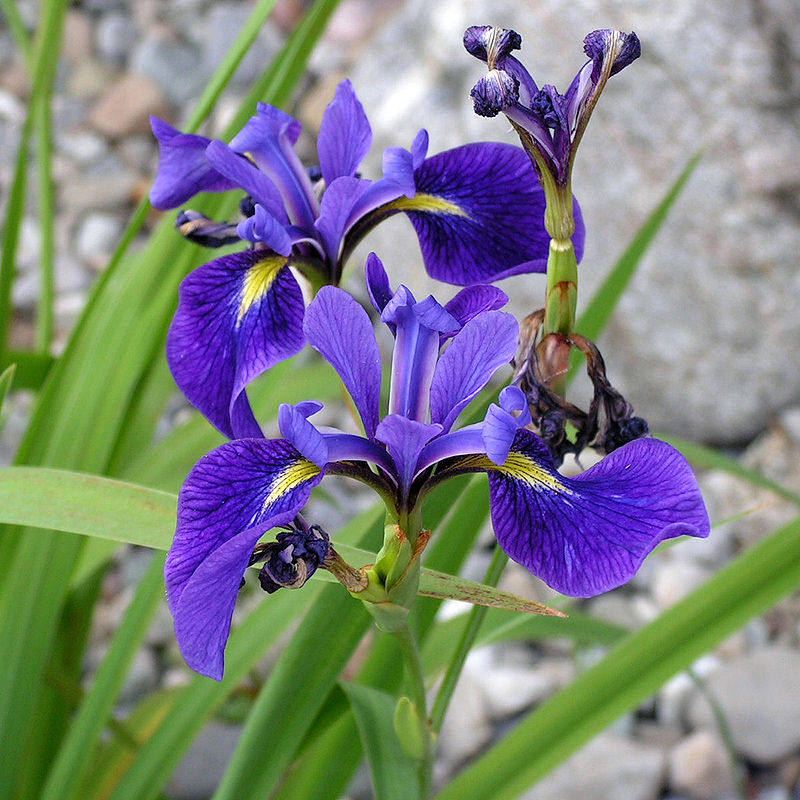
\includegraphics[scale=0.2]{versicolour}
    \caption{Iris Versicolour}
    \label{fig:versicolour}
\end{figure}
\begin{figure}
    \centering
    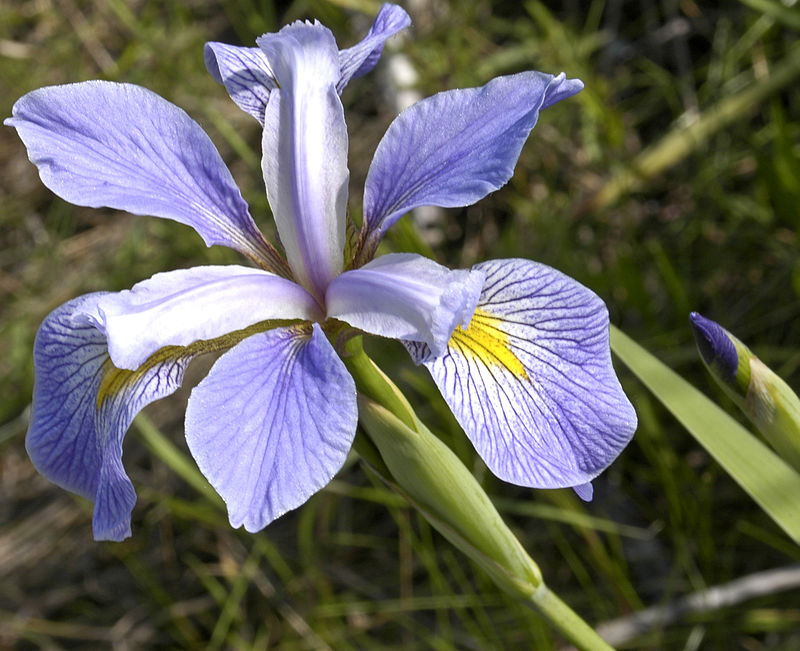
\includegraphics{virginica}
    \caption{Iris Virginica}
    \label{fig:virginica}
\end{figure}

\section{History of the dataset}
The dataset was introduced by Ronald Fischer in 1936 in his paper "The use of multiple measurements in taxonomic problems" ~\cite{setosa}. It is currently the most popular dataset in the UCI Machine Learning repository ~\cite{uci}
\section{Attribute information}
The dataset contains the following attributes ~\cite{iris}:
\begin{enumerate}
    \item Sepal length in cm
    \item Sepal width in cm 
    \item Petal length in cm 
    \item Petal width in cm
    \item Class - one of Iris Setosa, Iris Versicolour, Iris Virginica
\end{enumerate}
\section{First look at the dataset}
The dataset contains 150 records, with 50 for each class. The attributes sepal length, sepal width, petal length and petal width vary between 0 and 8. There are no missing values.

\chapter{Analyze the data}
\section{Handling missing values}
Since there are no missing values, we do not need to take actions to handle the missing values
\section{Balancing classes}
The classes are perfectly balanced, so we do not need Kappa metrics or anything like this.
\section{Normalization and standardization}
All attribute types are numeric, but they seem to take on values in slightly different intervals. Normalization or standardization may be beneficial.
\section{Descriptive statistics}
Both sepallength and sepalwidth seem to be normally distributed - see fig \ref{fig:sepal}, which means that Logistic Regresson is a good candidate, since it assumes normal distribution of the attributes. There seems to be a good separation between classes for petallength and petalwidth - see fig \ref{fig:plot_matrix}, so we should expect that a model with high accuracy exists and since SVM tries to separate the data with a line, SVM is probably an interesting choice, as are trees. Since a point is usually surrounded by points of the same class, k-nearest neighbour and other lazy methods seem like a good candidate. If we always predict the majority class, we get an accuracy of 32\%, so we should definitely aim for more than that baseline.
\begin{figure}
    \centering
    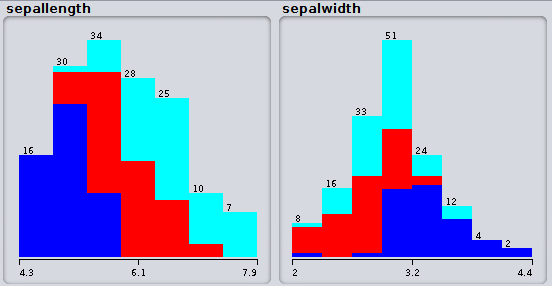
\includegraphics[scale=0.8]{sepal}
    \caption{Sepal attributes distribution}
    \label{fig:sepal}
\end{figure}
\begin{figure}
    \centering
    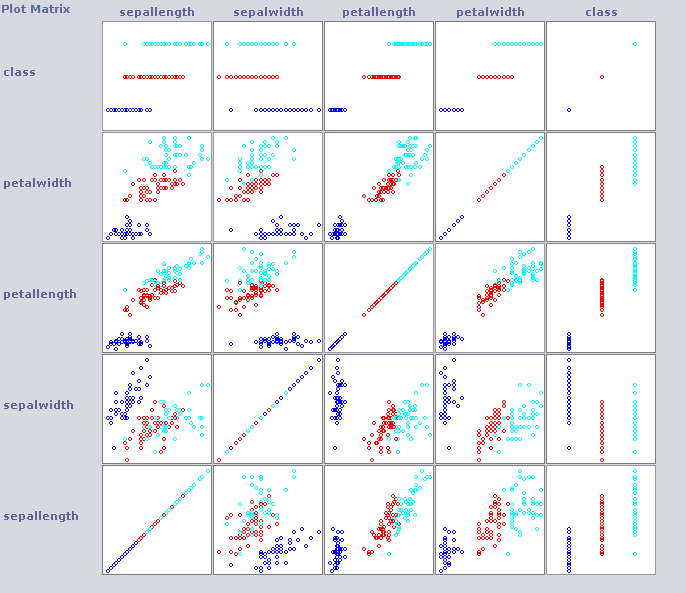
\includegraphics[scale=0.6]{plot_matrix}
    \caption{Separations per attribute of the classes}
    \label{fig:plot_matrix}
\end{figure}

\chapter{Prepare data}
We will describe the different views of the dataset that we will use in future experiments.
\section{Raw view of the dataset}
This is the way we downloaded it from the UCI Machine Learning dataset repository
\section{Normalized view of the dataset}
This is the raw dataset after normalizing all attributes, so that all attributes are now between 0 and 1.
\section{Standardized view of the dataset}
This is the raw dataset after standardizing all attributes, so that the mean of all attributes is now 0 and the standart deviation is 1.
\section{Dataset after feature selection}
This is the raw dataset with only petallength and petalwidth. Visually, they seem to separate the classes very well. Also, after running CFS and evaluating on the subsets and using greedy stepwise for search method, we get a result that petallength and petalwidth should be selected.

\chapter{Evaluate algorithms}
\section{Initial experiment design}
On the datasets in previous chapter, we will run the following algorithms:
\begin{enumerate}
    \item Logistic regression with ridge parameter 1.0E-8 without conjugate gradient descent
    \item k-Nearest Neighbour with 3 neighbours without distance weighting
    \item Naive Bayes
    \item Multilayer Perceptron neural network with learning rate 0.3 and momentum 0.2
    \item Support vector machine using sequential minimal optimization for training and logistic regression for calibrator with polykernel and 0.001 tolerance parameter
    \item Decision tree - Pruned C4 decision tree
    \item Adaboost - with pruned C4 decision trees instead of decision stumps
    \item Random forest - to avoid potential overfitting of the decision tree
\end{enumerate}

We will use cross validation on 5 folds. Results are available in the Github Repository ~\cite{repo}. After running the experiment, we see no significant difference between the results in the different views of the dataset. We will therefore choose the dataset with only two attributes and run the expreriment again. We then see ~\cite{repo} that SVM gives the best result, followed by logistic regression and multilayer perceptron.
We will concentrate on tuning these three algorithms in the next chapter and selecting one of them

\chapter{Impove results}
\section{Experiment for improving result}
We will now run an experiment with slightly different parameters to find the optimal parameters and select a feasible model. The configurations is available in the Github reposiory ~\cite{repo}. After running the experiments, we see that the results are similar, but the SVM classifier is with highest accuracy 96.07\%, so we sill choose this algorithm.

\chapter{Present results}
The final Weka model is availble in the Github repository